%%%%%%%%%%%%%%%%%%%%%%%%%%%%%%%%%%%%%%%%%

\chapter{The LANL nEDM experiment}\label{chap:LANL_nEDM}

%%%%%%%%%%%%%%%%%%%%%%%%%%%%%%%%%%%%%%%%%

At the Los Alamos National Laboratory (LANL), a solid deuterium (SD$_2$) based superthermal UCN source coupled to a spallation target has been providing UCN to experiments for the last 20 years (Fig.~\ref{fig:AreaB_schematic}). The UCN source (Sec.~\ref{sec:lanl_ucn_source}) was upgraded to host a new nEDM experiment that will use Ramsey's method of separated oscillatory fields to search for the nEDM with an uncertainty goal of $\delta \gls*{d_n} = 2.7\times 10^{-27}$~$e\cdot\text{cm}$ (Sec.~\ref{sec:lanl_nedm_uncertainty}).

The final LANL nEDM experiment will include features such as:
%
\begin{itemize}
    \item Two precession chambers (Sec.~\ref{sec:precession_chambers})
    \item Simultaneous spin analyzers (Sec.~\ref{sec:spin_flipper_analyzer})
    \item An external array of optically pumped magnetometers (Sec.~\ref{sec:magnetic_field_req})
    \item A $\ce{^{199}Hg}$ comagnetometer (Sec.~\ref{sec:199hg_comag}) and external $\ce{^{199}Hg}$ magnetometers
\end{itemize}

%%%%%%%%%%%%%%%%%%%%%%%%%%%%%%%%%%%%%%%%%

\section{Principles of an nEDM measurement}\label{sec:principles_nEDM}

%%%%%%%%%%%%%%%%%%%%%%%%%%%%%%%%%%%%%%%%%

A measurement cycle in the envisioned LANL nEDM experiment consists of the following steps: 
%
\begin{enumerate}
    \item Polarized \ucn are loaded into precession cell(s), in a region where a static magnetic $\vv{B}_0$ and electric field $\vv{E}$ are applied. $\vv{B}_0$ and $\vv{E}$ are in either a parallel ($\uparrow\uparrow$) or antiparallel ($\uparrow\downarrow$) configuration.
    \item The Ramsey sequence (Sec.~\ref{sec:ramsey-method}) is applied to generate a point on a Ramsey fringe, which is necessary for determination of UCN precession frequency in both parallel and antiparallel configurations.
    \item \ucn are unloaded from the precession cell(s) to be detected and to have their final spin state analyzed.
\end{enumerate}
%
Measurement cycles are repeated many times to minimize statistical uncertainty (Sec.~\ref{sec:figure_of_merit}). In the absence of any systematic effects, any difference in neutron precession frequency $\omega_\text{n}$ between the $\vv{B}_0\uparrow\uparrow\vv{E}$ and $\vv{B}_0\uparrow\downarrow\vv{E}$ configurations indicates the existence of a nonzero electric dipole moment \gls*{d_n}. This is written as
%
\begin{gather}
    \omega_\text{n}^{\uparrow\uparrow} - \omega_\text{n}^{\uparrow\downarrow} = -\frac{4\gls*{d_n}E}{\hbar}\label{eq:delta_omega_dipole_relation}
\end{gather}
%
where
%
\begin{align}
    \hbar \omega_\text{n}^{\uparrow\uparrow} &= -2\gls{mu_n}B_0 - 2\gls*{d_n}E\\
    \hbar \omega_\text{n}^{\uparrow\downarrow} &= -2\gls{mu_n}B_0 + 2\gls*{d_n}E
\end{align}
%
In the case where $B_0$ and $E$ differ between configurations,
%
\begin{gather}
    \gls*{d_n}=\frac{\hbar(\omega_\text{n}^{\uparrow\uparrow} - \omega_\text{n}^{\uparrow\downarrow})-2\gls{mu_n}(B_0^{\uparrow\uparrow} - B_0^{\uparrow\downarrow})}{2\hbar(E^{\uparrow\uparrow} - E^{\uparrow\downarrow})}
\end{gather}
%
\begin{figure}
    \centering
    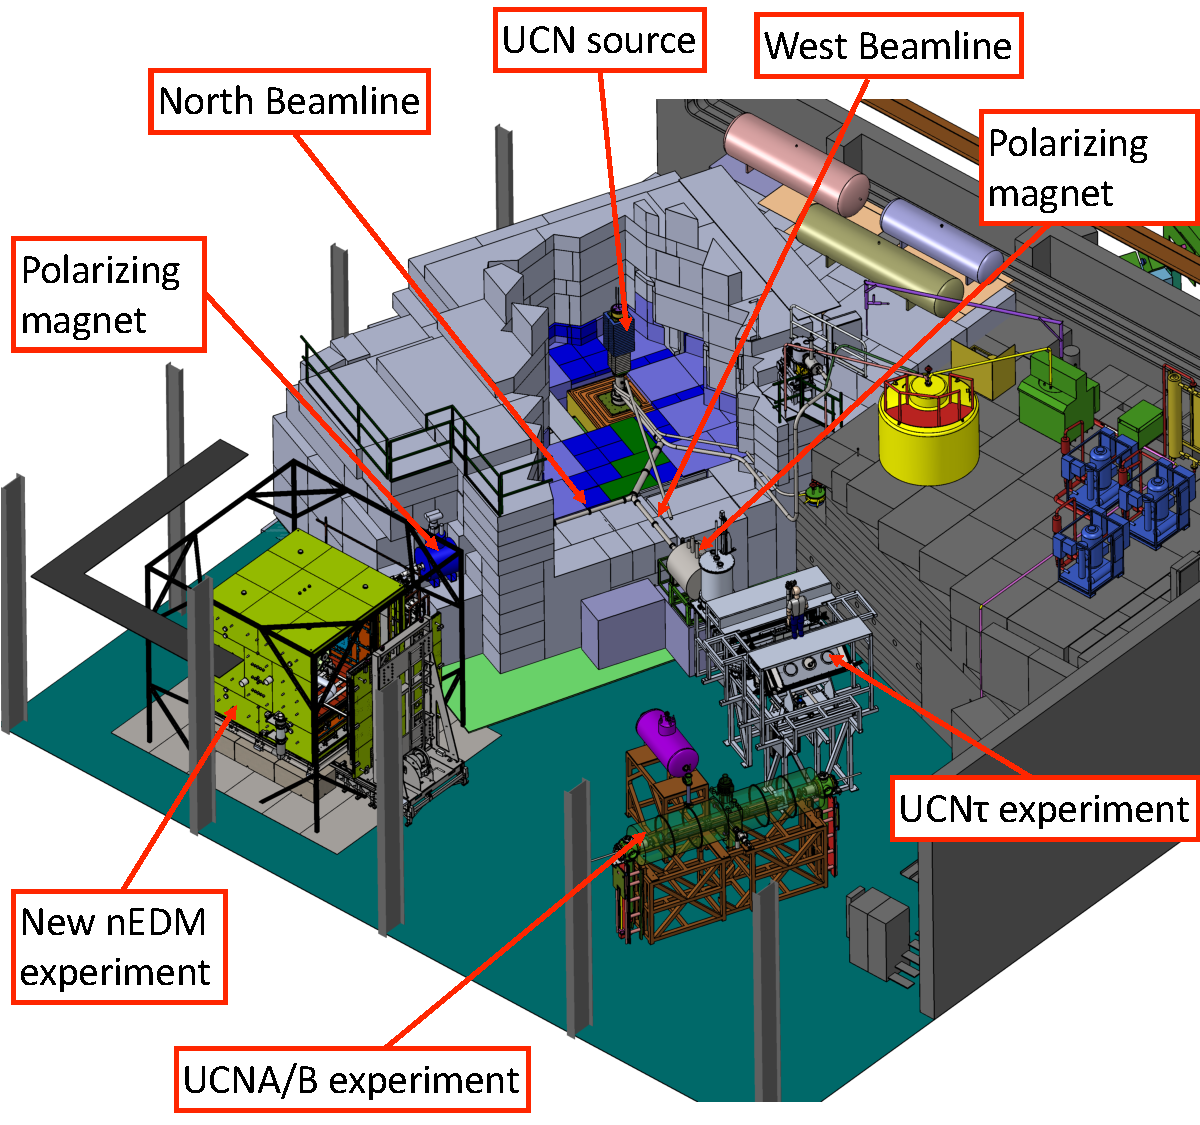
\includegraphics[width=0.6 \textwidth]{AreaB_v3.pdf}
    \caption{Schematic of the experimental area at the LANL UCN facility}
    \label{fig:AreaB_schematic}
\end{figure}

%%%%%%%%%%%%%%%%%%%%%%%%%%%%%%%%%%%%%%%%%

\section{Statistical uncertainty figure of merit}\label{sec:figure_of_merit}

%%%%%%%%%%%%%%%%%%%%%%%%%%%%%%%%%%%%%%%%%

Equation~7.28 from Ref.~\cite{golubUCN} gives the number of neutrons counted in a single Ramsey sequence as
%
\begin{gather}
    N_\text{R}(\Delta \omega) = N \left( 1 - \gls*{alpha} \cos \,\Delta \omega \, \gls*{T_fp} \right)/2
\end{gather}
%
where \gls*{alpha} is the spin contrast of a Ramsey fringe, defined by Eq.~(\ref{eq:alpha}), and $\gls*{T_fp}$ is the free precession period of the Ramsey method. A nonzero nEDM causes an interaction with $\vv{E}$ that produces a precession frequency shift $\Delta\omega=\omega-\omega_0$, where $\omega$ is the applied RF frequency and $\omega_0$ is defined by Eq.~(\ref{eq:larmor_freq}). 

To maximize sensitivity to small shifts in the resonant frequency, we examine where the slope of the central fringe is largest
%
\begin{gather}
    \frac{\partial N_\text{R}(\Delta \omega)}{\partial \, \Delta \omega} = N \frac{\alpha}{2} \gls*{T_fp} \sin \, \Delta \omega \, \gls*{T_fp} \label{eq:slope_ramsey}
\end{gather}
%
The error of $\Delta \omega$ is given by
%
\begin{gather}
    \sigma(\Delta \omega) = \frac{\partial \, \Delta \omega}{\partial N_\text{R}(\Delta \omega)}\delta N_\text{R}(\Delta \omega) = \frac{\partial \, \Delta \omega}{\partial N_\text{R}(\Delta \omega)} \sqrt{N}
    \label{eq:sigma_delta_omega}
\end{gather}
%
Using Eq.~(\ref{eq:slope_ramsey}) where $\Delta \omega \, \gls*{T_fp} = \pi/2$ (for the largest slope), Eq.~(\ref{eq:sigma_delta_omega}) becomes
%
\begin{gather}
    \sigma(\Delta \omega) = \frac{2}{\gls*{alpha} \gls*{T_fp} \sqrt{N}}
\end{gather}
%
From reversal of the electric field, Eq.~(\ref{eq:delta_omega_dipole_relation}), we remove the dependence on $\Delta\omega$ to obtain
%
\begin{gather}
    \sigma_{\gls*{d_n}} = \frac{\hbar}{2\gls*{alpha} E \gls*{T_fp} \sqrt{N}}\label{eq:figure_of_merit}
\end{gather}
%
This is the figure of merit for an nEDM experiment using the Ramsey method. \gls{hbar} is Planck’s constant, \gls{alpha} is a factor describing the spin contrast of a Ramsey fringe, $N$ is the number of the detected UCN, and $E$ is the strength of the applied electric field.

%%%%%%%%%%%%%%%%%%%%%%%%%%%%%%%%%%%%%%%%%

\subsection
{
    \texorpdfstring{Statistical Uncertainty of the \acrshort{lanl} \acrshort{nedm}}
                    {Statistical Uncertainty of the LANL nEDM}\label{sec:lanl_nedm_uncertainty}
}

%%%%%%%%%%%%%%%%%%%%%%%%%%%%%%%%%%%%%%%%%

The nominal run parameters for the LANL nEDM are $\gls*{T_fp}=180\text{ s and } E=12\text{ kV/cm}$. As will be shown in Chap.~\ref{chap:north_beamline_paper}, we have measured $N=60\,000\text{ counts per cell}$. We let $\gls*{alpha}=0.8$, as was achieved in Ref.~\cite{ABE20}.

Using Eq.~(\ref{eq:figure_of_merit}), the uncertainty per cell per run is $7.8 \times 10^{-25}e\cdot\text{cm}$. For a full day of measurements (assuming a \qty{300}{\s} duty cycle with two precession cells), we have $N_\text{day}=2\times60\,000\times86\,400\text{ (seconds in a day)}/300$ and $\sigma_{\gls*{d_n}}=3.24\times10^{-26}e\cdot\text{cm}$. A year of continuous running gives $N_\text{year}=365\times N_\text{day}$ and $\sigma_{\gls*{d_n}}=1.7\times10^{-27}e\cdot\text{cm}$. At a 90\% confidence level, the uncertainty is multiplied by an additional factor of $1.6$, giving
%
\begin{gather}
    \sigma_{\gls*{d_n}}=2.71\times10^{-27}e\cdot\text{cm (90\% \acrshort{cl})}
\end{gather}
%
Accounting for the production schedule at LANL, this uncertainty would be reached in 5 calendar years.

%%%%%%%%%%%%%%%%%%%%%%%%%%%%%%%%%%%%%%%%%

\section
{
    \texorpdfstring{UCN production at \acrshort{lanl}}
                   {UCN production at LANL}
}\label{sec:lanl_ucn_source}

%%%%%%%%%%%%%%%%%%%%%%%%%%%%%%%%%%%%%%%%%

At LANL, neutrons are produced by a pulsed \qty{800}{M\eV} proton beam incident on a tungsten target, which is surrounded by ambient temperature beryllium and graphite. The spallation neutrons are cooled by polyethylene bead moderators to cold neutrons, and are then converted to UCN by downscattering within an SD$_2$ crystal~\cite{saunders_performance_2013}.

As in Fig.~\ref{fig:lanl_ucn_source}, UCN leaving the SD$_2$ crystal are directed upwards along a \qty{1}{\meter} vertical guide coated in $\ce{^{58}Ni}$, to account for a Snell's law \qty{100}{\nano\eV} boost (Sec.~\ref{sec:ucn_reflection_transmission}). The UCN are then transported \qty{6}{\meter} along a horizontal NiP coated stainless steel guide to the exit of the biological shield~\cite{ito_performance_2018}.

A butterfly valve near the bottom of the vertical guide reduces the probability of UCN returning to the SD$_2$ and being absorbed. The valve is open while proton beam pulses are delivered to the spallation target and closed otherwise. The proton current from the accelerator is delivered in packets of 10 pulses, of pulse width \qty{625}{\micro\s} at \qty{20}{\hertz}, with a gap between packets of \qty{5}{\s}. The average current delivered to the target is $\sim\qty{9}{\micro A}$.

In a 2017 source upgrade, the cryogenic insert, which housed the SD$_2$ converter as well as the cold neutron moderator, was replaced with an improved design. The upgrade produced a factor of four increase in UCN density. UCN density measured at the exit of the biological shield was $\qty{184(32)}{UCN\per \cm^3}$, and polarized UCN density stored in an external chamber was $\qty{39(7)}{UCN\per \cm^3}$~\cite{ito_performance_2018}.

With the upgrade, a new UCN beamline (called the North Beamline) was constructed for the new nEDM experiment (Fig.~\ref{fig:AreaB_schematic}). Measurements and analysis characterizing the performance of the North Beamline are presented in Chap.~\ref{chap:north_beamline_paper}.

\begin{figure}
    \centering
    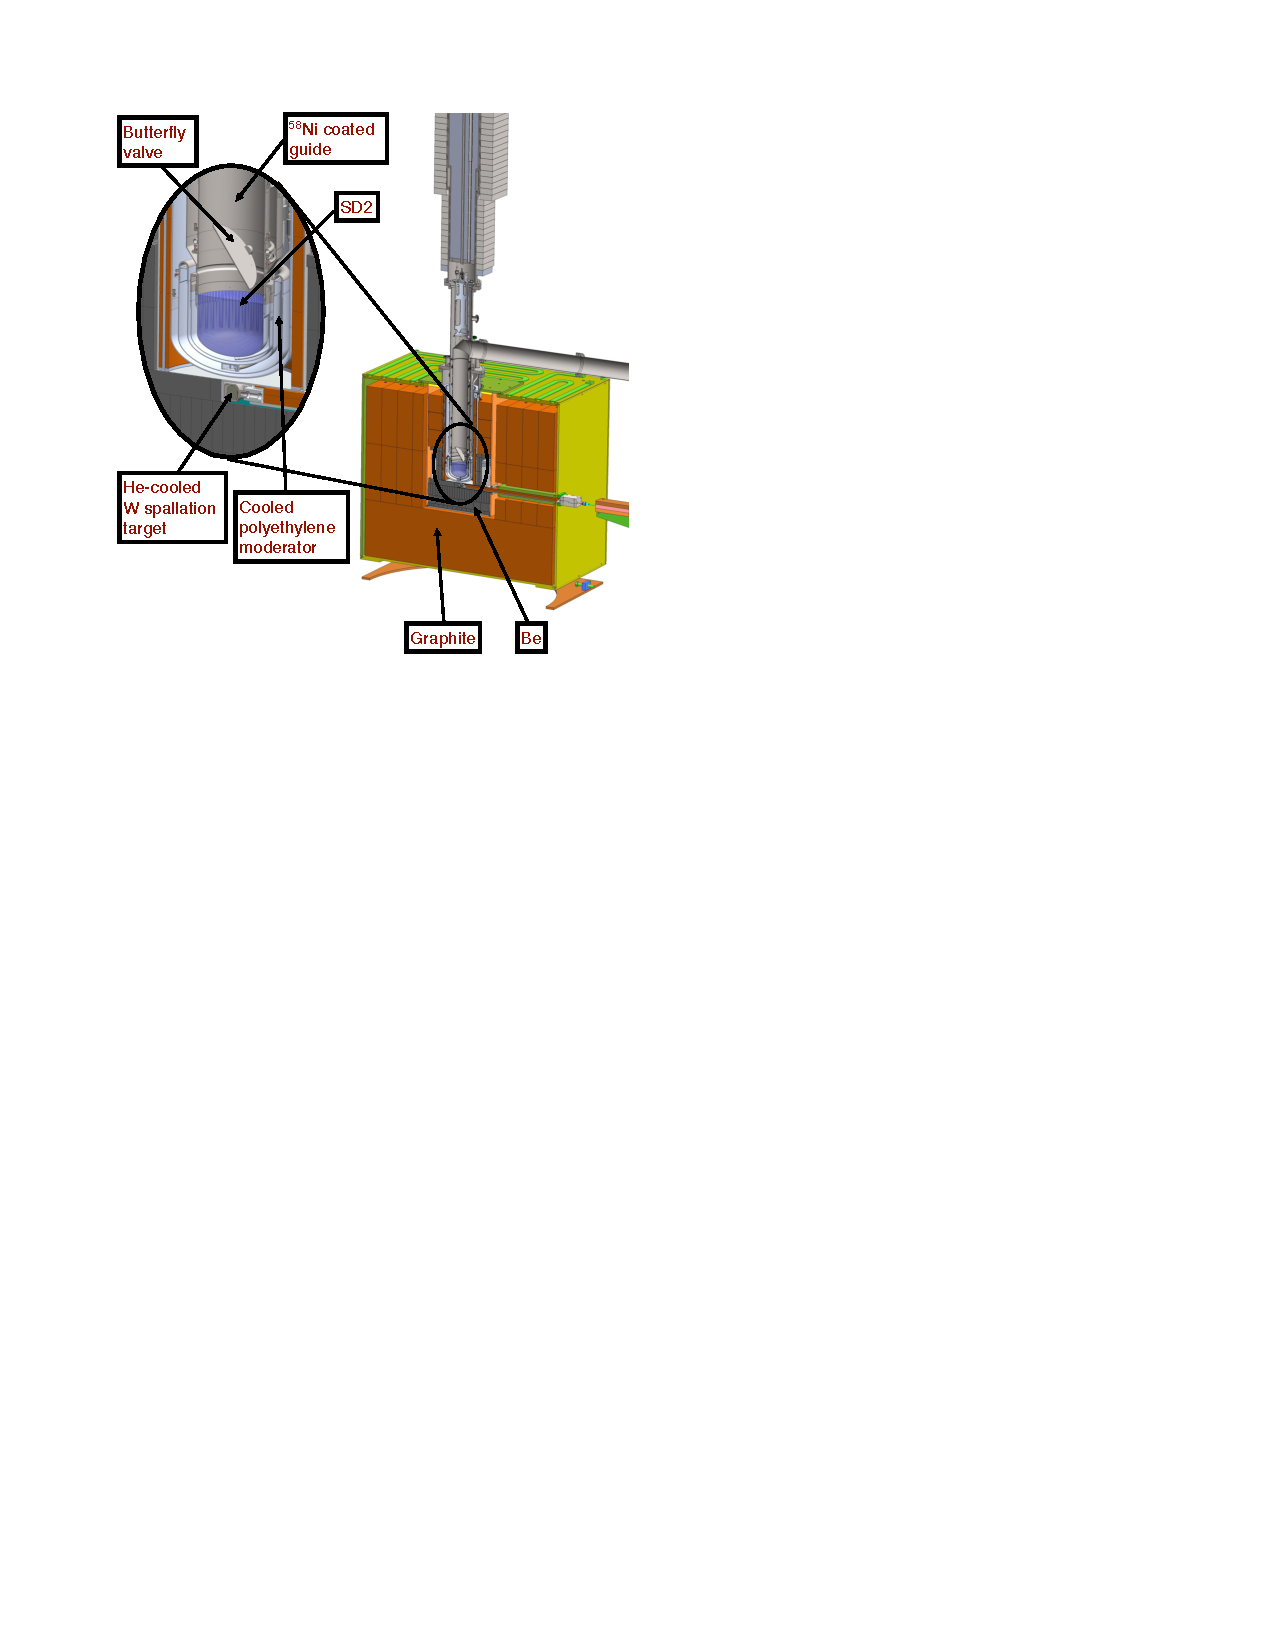
\includegraphics[width=0.45 \textwidth]{figures/lanl_ucn_source.pdf}
    \caption[Cutaway view of the LANL UCN source]
    {Cutaway view of the LANL UCN source. Image from Ref.~\cite{ito_performance_2018}}
    \label{fig:lanl_ucn_source}
\end{figure}


%%%%%%%%%%%%%%%%%%%%%%%%%%%%%%%%%%%%%%%%%

\section
{
    Magnetic field requirements\label{sec:magnetic_field_req}
}

%%%%%%%%%%%%%%%%%%%%%%%%%%%%%%%%%%%%%%%%%

%%%%%%%%%%%%%%%%%%%%%%%%%%%%%%%%%%%%%%%%%

\subsection
{
    \texorpdfstring{$\ce{^{199}Hg}$ Comagnetometer}
                    {199Hg Comagnetometer}\label{sec:199hg_comag}
}

%%%%%%%%%%%%%%%%%%%%%%%%%%%%%%%%%%%%%%%%%

%%%%%%%%%%%%%%%%%%%%%%%%%%%%%%%%%%%%%%%%%

\subsection
{
    \texorpdfstring{$v\times E$ motional effects}
                    {v x E motional effects}\label{sec:v_cross_E}
}

%%%%%%%%%%%%%%%%%%%%%%%%%%%%%%%%%%%%%%%%%

Geometric phase

%%%%%%%%%%%%%%%%%%%%%%%%%%%%%%%%%%%%%%%%%

\subsection{Magnetically Shielded Room}

%%%%%%%%%%%%%%%%%%%%%%%%%%%%%%%%%%%%%%%%%

%%%%%%%%%%%%%%%%%%%%%%%%%%%%%%%%%%%%%%%%%

\subsection{Performance as a function of ambient temperature}

%%%%%%%%%%%%%%%%%%%%%%%%%%%%%%%%%%%%%%%%%

\comment{Allan Variance}

%%%%%%%%%%%%%%%%%%%%%%%%%%%%%%%%%%%%%%%%%

\subsection{Static and clamped modes of the MSR door}

%%%%%%%%%%%%%%%%%%%%%%%%%%%%%%%%%%%%%%%%%

%%%%%%%%%%%%%%%%%%%%%%%%%%%%%%%%%%%%%%%%%

\subsection{External field active compensation}

%%%%%%%%%%%%%%%%%%%%%%%%%%%%%%%%%%%%%%%%%

%%%%%%%%%%%%%%%%%%%%%%%%%%%%%%%%%%%%%%%%%

\subsection{Transport coils}

%%%%%%%%%%%%%%%%%%%%%%%%%%%%%%%%%%%%%%%%%

%%%%%%%%%%%%%%%%%%%%%%%%%%%%%%%%%%%%%%%%%

\section{Polarizing magnet}\label{sec:PM_description}

%%%%%%%%%%%%%%%%%%%%%%%%%%%%%%%%%%%%%%%%%

A \qty{5}{\tesla}, horizontal warm bore, superconducting magnet by American Magnetics Inc. is used as a polarizing magnet (\acrshort*{pm}). The PM field filters UCN spins, acting as a potential barrier that rejects low-field seeking UCN below \qty{300}{\nano\eV} and a potential well that passes high-field seeking UCN (Sec.~\ref{sec:ucn_polarizers}). 

A \qty{0.1}{\milli\meter} thick Al97 Mg3 alloy foil (similar in tensile strength to 6061-T6), termed the ``PM window," is located in the beamline at the center of the PM field region. This is used to separate the UCN source vacuum from the measurement apparatus vacuum, as the source vacuum can be routinely filled with D$_2$ gas (e.g. while D$_2$ is being drawn from a storage tank to be frozen or while SD$_2$ is being reconditioned). The magnetic potential of the PM overwhelms the neutron optical potential of the window (\qty{54}{\nano\eV} \cite{golubUCN}). The effect of the window on the transmission of UCN is discussed in detail in Sec.~\ref{sec:analysis}.

%%%%%%%%%%%%%%%%%%%%%%%%%%%%%%%%%%%%%%%%%

\section{Spin flipper and analyzers}\label{sec:spin_flipper_analyzer}

%%%%%%%%%%%%%%%%%%%%%%%%%%%%%%%%%%%%%%%%%

Neutron spin analyzers in the LANL nEDM are 10 layer polarizers made of iron and silicon located immediately above neutron detectors (see Ref.~\cite{ThorstenThesis} for layer structure details). When magnetized with a ($\sim \qty{10}{mT}$) field from permanent magnets, the multi-layer polarizer preferentially transmits high-field seeking UCN and rejects low-field seeking UCN with an analyzing power of $99.3^{+0.7}_{-2.4}\%$~\cite{ThorstenThesis}.

Note that it is not clear if the neutron energy spectrum under which Ref.~\cite{ThorstenThesis} is consistent with the LANL nEDM neutron spectrum. Reference~\cite{afach_device_2015} quotes an analyzing power of 95\% for a different but similar analyzing foil for an energy range of 90~neV to 330~neV, which includes the energy range of the UCN at the analyzing foil for the experiment reported in Sec.~\ref{sec:analysis}.

Additionally, an adiabatic fast passage (\acrshort{afp}) spin flipper coil, located upstream of the spin analyzer, is used to provide the option of spin flipping UCN (Sec.~\ref{sec:afp}). A schematic of the analyzer system is illustrated in Fig.~\ref{fig:SpinAnalyzer}.

\begin{figure}
    \centering
    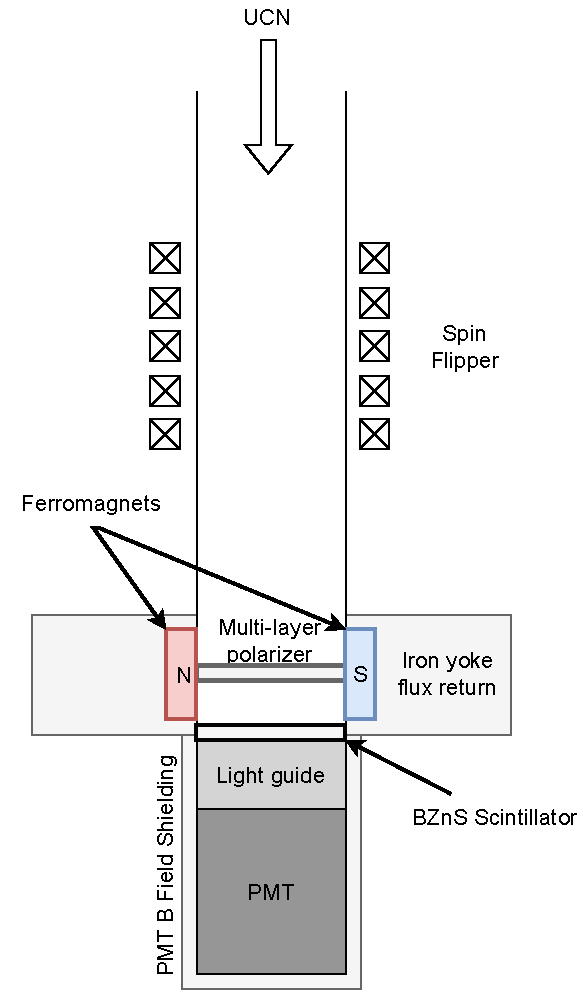
\includegraphics[width=5cm]{spinAnalyzer.pdf}
    \caption{Schematic of the adiabatic fast passage (\acrshort{afp}) spin flipper, spin analyzer, and UCN drop detector}
    \label{fig:SpinAnalyzer}
\end{figure}

%%%%%%%%%%%%%%%%%%%%%%%%%%%%%%%%%%%%%%%%%

\section{UCN detectors}

%%%%%%%%%%%%%%%%%%%%%%%%%%%%%%%%%%%%%%%%%

$\ce{^{10}B}$ coated ZnS:Ag scintillator films are used for UCN detection \cite{jeph_b10_2011}. UCN are captured on the top layer of $\ce{^{10}B}$, and reaction products ($^4$He and/or $^7$Li) from the $\ce{^{10}B}(\text{n},\alpha)^7\text{Li}$ neutron capture reaction are detected in the ZnS:Ag layer. The resulting scintillation light is then detected by a photomultiplier tube (\acrshort*{pmt}) or Si photomultiplier (\acrshort*{sipm})

%%%%%%%%%%%%%%%%%%%%%%%%%%%%%%%%%%%%%%%%%

\section{UCN switchers}

%%%%%%%%%%%%%%%%%%%%%%%%%%%%%%%%%%%%%%%%%

%%%%%%%%%%%%%%%%%%%%%%%%%%%%%%%%%%%%%%%%%

\section{Vacuum chamber}

%%%%%%%%%%%%%%%%%%%%%%%%%%%%%%%%%%%%%%%%%

%%%%%%%%%%%%%%%%%%%%%%%%%%%%%%%%%%%%%%%%%

\section{Precession chambers}\label{sec:precession_chambers}

%%%%%%%%%%%%%%%%%%%%%%%%%%%%%%%%%%%%%%%%%

%%%%%%%%%%%%%%%%%%%%%%%%%%%%%%%%%%%%%%%%%

\subsection{dPS coating procedure}

%%%%%%%%%%%%%%%%%%%%%%%%%%%%%%%%%%%%%%%%%


%%%%%%%%%%%%%%%%%%%%%%%%%%%%%%%%%%%%%%%%%

\section{Scanning for magnetic contamination}

%%%%%%%%%%%%%%%%%%%%%%%%%%%%%%%%%%%%%%%%%